%%%%%%%%%%%%%%%%%%%%%%% file template.tex %%%%%%%%%%%%%%%%%%%%%%%%%
%
% This is a general template file for the LaTeX package SVJour3
% for Springer journals.          Springer Heidelberg 2010/09/16
%
% Copy it to a new file with a new name and use it as the basis
% for your article. Delete % signs as needed.
%
% This template includes a few options for different layouts and
% content for various journals. Please consult a previous issue of
% your journal as needed.
%
%%%%%%%%%%%%%%%%%%%%%%%%%%%%%%%%%%%%%%%%%%%%%%%%%%%%%%%%%%%%%%%%%%%
%
% First comes an example EPS file -- just ignore it and
% proceed on the \documentclass line
% your LaTeX will extract the file if required
\begin{filecontents*}{example.eps}
%!PS-Adobe-3.0 EPSF-3.0
%%BoundingBox: 19 19 221 221
%%CreationDate: Mon Sep 29 1997
%%Creator: programmed by hand (JK)
%%EndComments
gsave
newpath
  20 20 moveto
  20 220 lineto
  220 220 lineto
  220 20 lineto
closepath
2 setlinewidth
gsave
  .4 setgray fill
grestore
stroke
grestore
\end{filecontents*}
%
\RequirePackage{fix-cm}
%
%\documentclass{svjour3}                     % onecolumn (standard format)
%\documentclass[smallcondensed]{svjour3}     % onecolumn (ditto)
\documentclass[smallextended]{svjour3}       % onecolumn (second format)
%\documentclass[twocolumn]{svjour3}          % twocolumn
%
\smartqed  % flush right qed marks, e.g. at end of proof
%
\usepackage{graphicx}
\usepackage{natbib}

%
% \usepackage{mathptmx}      % use Times fonts if available on your TeX system
%
% insert here the call for the packages your document requires
%\usepackage{latexsym}
% etc.
%
% please place your own definitions here and don't use \def but
% \newcommand{}{}
%
% Insert the name of "your journal" with
% \journalname{myjournal}
%
\begin{document}

\title{Sex differences in mobility and spatial cognition%\thanks{Grants or other notes
%about the article that should go on the front page should be
%placed here. General acknowledgments should be placed at the end of the article.}
}
\subtitle{A test or the fertility and mothering hypothesis in northwestern Namibia}

%\titlerunning{Short form of title}        % if too long for running head

\author{Layne Vashro, Lace Padilla, Elizabeth Cashdan
}

%\authorrunning{Short form of author list} % if too long for running head

\institute{L. Vashro \at
              270 South 1400 East, Salt Lake City, UT 84112 \\
              Tel.: +001 (801) 581 6251\\
              \email{layne.vashro@anthro.utah.edu}           %  \\
}

\date{Received: date / Accepted: date}
% The correct dates will be entered by the editor


\maketitle

\begin{abstract}
Insert your abstract here. Include keywords, PACS and mathematical
subject classification numbers as needed.
\keywords{First keyword \and Second keyword \and More}
% \PACS{PACS code1 \and PACS code2 \and more}
% \subclass{MSC code1 \and MSC code2 \and more}
\end{abstract}

\section{Introduction}
\label{sec:1}
Researchers consistently find  that men perform better than women in certain spatial-cognitive and navigational tasks.  These differences are well-documented in Western industrialized societies and have increasingly been replicated cross-culturally.  Evolutionary psychologists have put forward several distinct theories that link these sex differences to further differences in traveling long distances and into unfamiliar environments.  In most of these theories, past selection favored the males who could travel more safely and efficiently which required superior navigation ability and the spatial-cognitive traits that facilitate it \citep{jones2003evolution}.  The key point of disagreement among these arguments is simply the presumed payoff of that travel, whether it is mates \citep{gaulin1992evolution}, hunting \citep{eals1994hunter}, or warfare \citep{geary1995sexual}.  However, one explanation for the sex differences in ranging, spatial cognition, and navigation ignores the payoffs to males and instead turns the focus on the fitness ramifications of women's long-distance mobility.  This ``fertility and mothering hypothesis'' put forward by \citet{sherry1997evolution} argues that the observed sex differences can be explained in terms of the potential costs to women traveling, particularly during key periods of reproduction \citep{ecuyer2004have}.

	\subsection{Fertility and mothering}
	\label{sec:1.1}
The fertility and mothering hypothesis highlights the relationship between women's performance on spatial tasks and hormones related to reproduction.  Women's performance in spatial-cognitive tasks that typically favor men is at its lowest in the middle of their menstrual cycle, possibly due to the concurrent peak in estrogen levels \citep{hampson1988reciprocal, hampson1990estrogen, mccormick2001menstrual, komnenich1978gonadal, hausmann2000sex}.  This interpretation is consistent with the improved performance in a mental rotation task among postmenopausal women given estrogen replacement therapy \citep{duka2000effects}, as well as studies linking estrogen to spatial ability in several non-human mammals \citep{fugger1998sex, lacreuse1999spatial, frye1995estrus}.  Assuming spatial ability is a necessary component of successful navigation, hormonal shifts that decease spatial ability should also inhibit travel.  The fertility and mothering hypothesis notes that ancestral women who avoided the risks and caloric costs of travel during key reproductive periods may have outcompeted those who did not \citep{sherry1997evolution}.  Following from this, women's diminished spatial ability is seen as an adaptive mechanism that pays by limiting travel.
	
Risky strategies tend to pay higher fitness dividends when variance in reproductive success among competitors is high \citep{darwin1871sexual, bateman1948intra, clutton1991sexual, clutton2007sexual}.  As is the case in many species, men's reproduction skews higher than women's \citep{trivers1972parental, wilson1985competitiveness}.  The constraints of women's extensive prepartum investment in offspring places a ceiling on potential reproduction, and in doing so limits the prospective bounty paid to risky strategies relative to men.  In addition to this common mammalian pattern, humans are a particularly altricial species.  Infants have an extended period of dependence, the burden of which falls predominantly on the mother in most societies.  Fitness calculations for men need to account for the potential loss of future offspring due to risky behavior, but at least in the subsistence societies that have been investigated, fathers' deaths do not endanger living children \citep{sear2008keeps}.  This is not the case for women, since the passing of a mother dramatically reduces any dependent children's likelihood of survival \citep{hill1996ache, sear2008keeps}.  

%The application of evolutionarily informed perspectives on risk has illuminated the discussion of sex-differences in violence, risky leisure activities, and even financial decision-making \citep{wilson1985competitiveness, wilson1997life, jianakoplos1998women}.

Travel away from home is risky behavior.  Large predators, snakes, interpersonal violence, inclement weather, exposure, falling rocks, and many other dangers are real concerns when navigating wild natural environments \citep{treves1999risk, pugh1980incidence, walker2001bioarchaeological}.  The nature of the risk has changed for many of us in today's world, but travel remains one of the riskier activities.  Travel related ``road injury'' is the seventh most common cause of death worldwide \citep{krug2000global}, and even in the United States traffic accidents are the second largest external cause of death \citep{sherry2010cdc}.  

In addition to the risks of travel, the fertility and mothering hypothesis also highlights the energetic costs of travel and how these trade off against the need to divert as many calories as possible towards reproduction.  With these concerns about the risks and energetic costs of travel in mind, the link between hormonal patterns associated with women's reproduction and the tools and desire to travel broadly presents an appealing evolutionary narrative.  However, the logical thread hangs on several assumptions about the relationship between women's reproductive life-history and cognition and mobility that need to be demonstrated.

	\subsection{Predictions}
	\label{sec:1.2}
This paper sets out to test a series of predictions drawn from the fertility and mothering hypothesis.  In some cases this means replicating well-established patterns in a population that faces navigational challenges more similar to those faced by ancestral humans.  In other cases, we offer the first test of predictions that underpin the fertility and mothering hypothesis and/or help distinguish it from alternative evolutionary theories explaining human sex differences across these traits.	
	
\paragraph{1. Men will demonstrate higher spatial-cognitive and navigational ability, report lower spatial anxiety, and travel more broadly.}\mbox{}\\

Men outperform women in specific measures of cognitive spatial ability \citep{sanders1982sex, shepard1971mental, eals1994hunter, lawton2010gender}.  This difference begins in infancy \citep{quinn2008sex, moore2008mental, levine1999early}, and is found in several non-human mammals \citep{javsarevic2012spatial, perdue2011sex, gaulin1986sex}.  Measures of navigational skill, especially those that tap into cues used in long-distance travel into unfamiliar environments also tend to favor men \citep{moffat1998navigation, bryant1982personality, galea1993sex, henrie1997gender}, though this difference is not as robust \citep{burke2012women, gilmartin1984comparing, montello1999comparison}.  Women also report higher levels of spatial anxiety than men and are less confident in their navigational ability \citep{devlin1995interactive, lawton1994gender, picucci2011besides}.  Finally, research across a broad spectrum of environmental and subsistence contexts finds that men occupy larger ranges than women \citep{ecuyer2004have, gaulin1988evolution, macdonald1999reproductive}.

This collection of sex-differences captures the empirical pattern that led researchers to posit the fertility and mothering hypothesis, as well as the other competing hypotheses noted above.  Previous work among the Twe and Tjimba found that these groups do indeed conform to this expected sex-difference in spatial cognition, navigation, and ranging \citep{vashro2014spatial}.  This study adds an improved measure of spatial-cognitive ability and a measure of spatial anxiety.

\paragraph{2.  Women's mobility and associated cognitive traits will increase (at least relative to men) following menopause.}\mbox{}\\

Unlike most mammals, human women may live an additional third of their lives following the cessation of fertility \citep{hawkes2003grandmothers}.  Women in this postmenopausal period are no longer primary care-providers, and thus should value risk aversion and energy conservation more similar to their male age-mates.  Following from the fertility and mothering hypothesis, this means postmenopausal women should be more mobile, less anxious, and perform better in spatial-cognitive tasks than reproductive-aged women, at least relative to same-aged men.  Previous research has failed to demonstrate any decrease in the sex-difference in performance on a mental rotation task, spatial memory task, or navigating virtual environments in humans \citep{willis1988gender, driscoll2005virtual, moffat2001age}, but one study does find the expected reduced sex difference with age in performance on a spatial memory task with among rhesus monkeys, \emph{Macaca mulatta} \cite{lacreuse1999spatial}.  This study compares postmenopausal and reproductive-aged women in measures of spatial ability, navigational ability, spatial anxiety, and mobility.    

%The decline in spatial ability and navigation with age appears to affect both men and women equally.  One early longitudinal study found no change in the magnitude of the sex difference in spatial ability in the transition from middle to old age\cite{willis1988gender}.  Another failed to find any interaction effect between sex and age in performance in a virtual water maze \cite{driscoll2005virtual}.  This same study found that the sex difference disappeared in ``middle'' as opposed to ``young'' or ``old'' adults.  However, this finding is difficult to interpret from the perspective of the fertility and parental hypothesis because the ``middle'' group spans age 40 to 59 which overlaps the expected ages of both pre and post menopausal women.  MOFFAT also finds no interaction in VWM!!  \cite{moffat2001age}
%This study compares postmenopausal and reproductive-aged women across these measures.  

%This pattern as been shown in rhesus monkeys, \emph{Macaca mulatta}, \cite{lacreuse1999spatial}. Longitudinal study found that the sex difference remained stable from middle into old age \cite{willis1988gender}

The fertility and mothering hypothesis makes a similar prediction about the comparison of reproductive-aged women and prepubescent girls, but we only included adult participants in this study.
  
\paragraph{3.  Reproductive-aged women's mobility and associated cognitive traits will decrease when they are pregnant or lactating}\mbox{}\\

Women cycle through a series of reproductive stages: mating (courtship, estrous), gestation, parturition, lactation, post-lactational parental care, and maternal recovery during their reproductive career \citep{gittleman1988energy}.  In a review of the fertility and mothering hypothesis, \citet{jones2003evolution} highlight gestation and lactation as particularly important periods for women to limit exposure to risk and caloric expenditure.  

%This emphasis on gestation and lactation is consistent with broader logic of the fertility and mothering hypothesis, but fits awkwardly with the core hormonal insights.  

Women's energy budgets increase by approximately 8-10\% during pregnancy, and 26\% postpartum.  Women manage this elevated demand through a combination of increased caloric intake, reduced movement, and in the case of lactation, by catabolizing fat stored during pregnancy \citep{dufour2002comparative}.  In addition to increased energetic demands, pregnant and postpartum women often report higher levels of anxiety \citep{heron2004course, wenzel2003prevalence}.  This is not a surprising pattern since any threats now necessarily extend to the dependent offspring as well.  Furthermore, environmental threats like spiders, scorpions, small mammalian predators, and exposure pose uniquely deadly threats to infants.  Among some of our closest primate relatives, including chimpanzees, \emph{Chimpanzee chimpanzee}, gorillas, \emph{Gorilla gorilla gorilla}, and baboons, \emph{Papio cynocephalus}, the threat of infanticidal non-paternal males constrains the movement of mothers with unweaned infants in a variety of ways \citep{collins1984infanticide, watts1989infanticide, smuts1992male, stokes2003female, watts2000infanticide}.  Male infanticide is rare in contemporary human societies, but may have been a realistic threat in our ancestral past, and other forms of sexual violence threaten women traveling alone in some societies \citep{gregor1987anxious}.

%\citep{woodfield1984embedded} pregnant women perform worse on embedded figures task

Assuming women's mobility and the cognitive traits that facilitate it respond facultatively to risk and energetic needs, pregnant and lactating women should be at the extreme in terms of limiting mobility and thus performance on spatial-cognitive and navigational tasks.  These women should also report higher levels of spatial anxiety than other women.  This study tests these predictions by comparing pregnant and postpartum Twe women to other Twe women of reproductive age.

\paragraph{4. Spatial cognition predicts women's range size.}\mbox{}\\

The fertility and parental care hypothesis predicts a positive correlation between \emph{women's} spatial ability and range size. Competing explanations for the male advantage in spatial cognition predict a positive correlation between \emph{men's} spatial ability and range size.  In each case, these arguments are agnostic to the relationship within the other sex; however, if spatial ability only predicts male range size it poses a challenge to the fertility and parental care hypothesis.  

One study demonstrated a positive correlation between spatial ability (measured using the Morris water maze task) and range size among male meadow voles, \emph{Microtus pennsylvanicus}, but did not look for a similar relationship among females \citep{spritzer2005influence}.  Two studies investigating this relationship in humans, one among urban Canadians and another among the Twe and Tjimba of northwestern Namibia, found a relationship between performance on the mental rotation task and range size for men but not women \citep{vashro2014spatial}.  However, the sample for the Namibian study was small and thus the lack of a relationship among women may be the result of Type II error.  This study attempts to replicate this finding among a similar population using an improved mental rotation task and a larger sample of participants. 

\section{Methods}
\label{sec:2}
	\subsection{Population}
Participants in this study live in the dry mountainous region near the Kunene River which separates northwestern Namibia and southwestern Angola.  This is a wild environment free of paved roads and large artificial structures.  None of the participants in the study own an automotive vehicle, and with the exception of occasionally hitch-hiking to the town, all travel is on foot (or sometimes by donkey).  Most participants report having become lost at some point in there lives.  The field researcher was present during two instances of a search party being called for a missing person.  In one case, an adolescent boy wandered too far during the day and could not find his way home by nightfall.  In the other case, an elderly man became lost traveling between two villages.  Many of the traditionally dangerous species of wildlife no longer live in the region \citep{viljoen1982distribution}, but people still list leopards and snakes as real threats to travelers, especially when passing through the mountains.  State police rarely patrol the region, but inter-personal violence is suppressed through tribal law and the threat of involving the Namibian authorities.  That said, violence is of some concern to people traveling outside their home region.  As an example, the field researcher visited one remote mountain village where a rapist had been targeting women who traveled unaccompanied to their gardens.

This study included all of the people living in the \emph{Ovizorowe} mountain valley in northwestern Namibia.  This valley is known as the home of the Twe ethnic group, but 32\% of the sample (41 participants) is drawn from Himba villages on the western and eastern-most ends.  For the purposes of this study, the most meaningful difference between these groups is that Himba men tend to own considerably more livestock than Twe men.  Men are responsible for bringing cattle to pasture in distant locations once the local supply of grass is depleted.  This results in a greater sex difference in mobility, at least for economic purposes, than is seen among the Twe.  Our samples captures a similar range of participants across the relevant demographic features from both the Twe and Himba.  The results reported below do not distinguish tribe membership and speak to the population of ``people living in the \emph{Ovizorowe} valley''.

Twe and Himba women do not have access to birth-control and a large proportion of their lives are spent either pregnant or breastfeeding.  Children are typically weaned at somewhere between 18 and 30 months old.  Most of the reproductive-aged women included in this study (56\%) reported that they were currently in the lactation stage of reproduction.  Unweaned children are almost always in contact with their mother, either actively feeding, strapped to her back while she works, or lying together in the shade while she rests.  Mothers are granted a brief reprieve from work immediately surrounding parturition, but afterwards are expected to continue their role in domestic production.

We recruited a total of 129 participants, including 65 men and 64 women for this study.  Intake interviews asked participants' age and reproductive status.  This allowed us to separate the participants into groups of ``postmenopausal'' (all women over 50 years of age, $n = 16$) and ``reproductive-aged'' (all women under 50 years of age, $n = 48$), then further subdivide the reproductive-aged women into ``pregnant'' ($n = 3$), ``lactating'' ($n = 27$), or ``other'' ($n = 18$).  The experimental items were split into two sessions, but we were not successful in recovering all of the participants for the second session.  Due to this, sample sizes vary by task as noted in the results below.

		\subsubsection{Spatial cognition}
		\label{sec:2.2.1}		
\paragraph{Mental rotation:}  This task is a computer-based adaptation of the Mental Rotation Test developed by \citep{shepard1971mental}.  Participants are shown two computer generated bodies rotated at 0, 60, 120, 180, 240, or 300 degrees on a two-dimensional axis.  One of the bodies has a left hand out-stretched while the other has a right arm out-stretched.  Participants are then asked to identify which of the two images matches a third body at the top of the screen with either a left or right hand out-stretched.  This task is repeated for 24 trials with the rotation of the correct image evenly distributed across the six possible degrees of rotation.  The task was designed using gaming software \citep{unity14} and presented to participants on a Toshiba 15.6" Touch-Screen laptop.  Measures of task performance include both accuracy across the 24 trials and the average amount of time needed to respond to each trial.

While most participants understood the task, it was clear that some did not. Before beginning the task, participants worked through a set of training stimuli consistent with the images used in the actual experiment.  Participants who failed to demonstrate understanding during this training were not asked to move on to the recorded trials.  Also due to the concern that some participants did not understand the task, we further removed any participants who scored below chance (50\%) across the 24 trials.  Finally, we removed all of the 0-degree trials before analysis, since responding to those trials does not require mentally rotating an image.

		\subsubsection{Navigation}
		\label{sec:2.2.2}
\paragraph{Real-world pointing:}  We used accuracy pointing to distant locations as a measure of navigation abilities. The task uses ten well-known locations with distances ranging from 10 to 130 kilometers.  Viewers were asked if they had visited each location. If they had, they were then asked to use the sight on a Brunton Pocket Transit International Compass to indicate the bearing to that location. This estimated bearing was then compared to the actual bearing to the location, and the absolute difference between them was recorded as the participant's error. Measurements were taken in locations that were free of objects that visually occluded participants' views (e.g. dense foliage and mountains).  The majority of participants had never visited three of the locations.  Before beginning the analysis, we removed points to these three locations and averaged across all of the remaining points for each participant.

		\subsubsection{Anxiety}
		\label{sec:2.2.3}
		
\paragraph{Spatial anxiety questionnaire:}  This questionnaire included four questions in the native Twe and Himba language of \emph{Otjiherero}.  These questions were inspired by items in the spatial anxiety scale developed by Carol Lawton \citep{lawton1994gender}.  The original questions were    we used a questionnaire that tested spatial anxiety in situations that required spatial and navigation skills, such as trying a new shortcut. Participants were presented with navigationally challenging scenarios then ask to indicate if they were concerned, sometimes concerned, or not concerned by the scenario.

	\subsection{Mobility}
	\label{sec:2.2.4}
	
\paragraph{Annual visiting interviews:}  Participants were asked to name each place away from their home village that they spent the night in the past year.  In addition, for each location they were asked who they traveled with, who they stayed with, and why they made the trip.  These data were used to calculate the number of unique locations visited by each participant in the past year.  In addition to this measure of ``annual range'', we also calculated the percentage of trips on which the participant was unaccompanied.  This additional measure is designed to account for the fact that solo traveling presents a unique navigational challenge, in that a person is unable to free-ride on the navigational skills of others.

\paragraph{Daily GPS tracking:}  Participants were given INSERT MODEL NAME GPS trackers to wear for three days.  In order to ensure recovery of the GPS devices, participants were asked to return them before leaving the village for more than one night.  This makes the daily mobility tracks a poor measure of travel into less familiar and thus risky areas, but does allow for a precise measure of daily movement as it relates to the energetic costs of local travel.  The analyses below use the net meters traveled by each participant on an average day. 

\section{Results}
\label{sec:3}
	\subsection{Sex differences}
	\label{sec:3.1}
Men responded more accurately, though not more quickly, than women to the mental rotation stimuli (see Table \ref{tab:sex}).  The real magnitude of this difference is likely larger than these results show, due to bias in the patterning of missing data.  Only 18.8\% of men were omitted from the analysis due to failure to demonstrate understanding compared to 28.3\% of women.  Assuming some correlation between spatial ability and ease of comprehending a spatial task, these analyses understate the sex difference.  

\begin{table}[h!]
\caption{Sex differences}
\label{tab:sex}  
\begin{tabular}{llllllll}
\hline\noalign{\smallskip}
& \multicolumn{2}{c}{Men} && \multicolumn{2}{c}{Women} && \\
Measure & \emph{N} & \emph{M(SD)} && \emph{N} & \emph{M(SD)} && \emph{p} \\
\noalign{\smallskip}\hline\noalign{\smallskip}
Mental rotation (accuracy) & 55 & 89.3\%(2.7\%) && 43 & 82.7\%(16.4\%) && .033 \\
Mental rotation (time) & 55 & 5.91(1.95) && 43 & 5.64(1.73) && .459 \\
Pointing error & 61 & 15.18$^{\circ}$(7.51$^{\circ}$) && 57 & 19.22$^{\circ}$(9.26$^{\circ}$) && .011 \\
Spatial anxiety & 27 & 2.29(0.57) && 27 & 2.64(0.37) && .010 \\
Annual visits & 42 & 4.29(4.18) && 45 & 2.02(1.59) && .002 \\
Solo visit \% & 40 & 46.4\%(38.7\%) && 40 & 24.2\%(37.1\%) && .011 \\
Daily mobility (km) & 20 & 8.75(5.49) && 18 & 4.38(2.59) && .004 \\
\noalign{\smallskip}\hline
\end{tabular}\par
\bigskip
Means and standard deviations for men and women in each of the listed measures. Final column gives the \emph{p-value} for a Chi-squared test comparing the two groups. 
\end{table}		  

Men also made smaller errors in the pointing accuracy task, self-reported lower spatial anxiety, visited more unique locations in the past year, traveled alone to a higher percentage of those locations, and traveled more than twice as far on a daily basis.  All of these differences are statistically significant (see Table \ref{tab:sex}).

% For one-column wide figures use
\begin{figure}[!htb]
  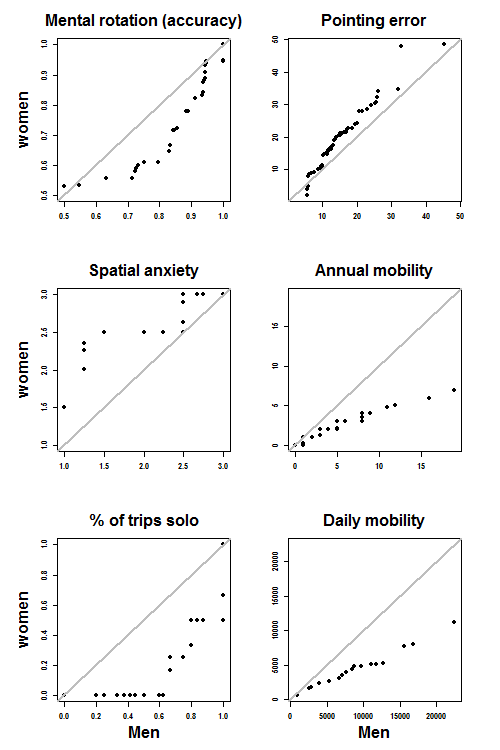
\includegraphics[width=0.75\textwidth]{QQ_sex}
\caption{Please write your figure caption here}
\label{fig:sex}       % Give a unique label
\end{figure}


	\subsection{Menopausal effects}
	\label{sec:3.2}
	
Postmenopausal women responded more slowly to the mental rotation task than reproductive-aged women, and were slightly less accurate (see Table \ref{tab:meno}).  Postmenopausal women were also much more likely than reproductive-aged women to fail to demonstrate sufficient understanding (61.4\% compared to 21.4\%), and thus not be included in the analysis.  The fertility and parental care hypothesis does not necessarily predict postmenopausal women will outperform younger reproductive-aged women, but it does expect the sex difference to be smaller among older participants.  However, comparing men above and below 50 years old, the older men performed worse than the younger men, but the difference is smaller than the decline seen among women (Accuracy decrease from 89.6\% to 86.7\% and reaction time increase from 5.7 to 7.6).  It does not look like women's spatial ability improves after menopause even accounting for general age-based decline shared with men.  

Unlike spatial ability, there is no meaningful difference between pre and postmenopausal women in pointing accuracy, nor is there is difference between older and younger men.

\begin{table}[h!]
\caption{Postmenopause}
\label{tab:meno}  
\begin{tabular}{llllllll}
\hline\noalign{\smallskip}
& \multicolumn{2}{c}{Postmenopausal} && \multicolumn{2}{c}{Reproductive-aged} && \\
Measure & \emph{N} & \emph{M(SD)} && \emph{N} & \emph{M(SD)} && \emph{p} \\
\noalign{\smallskip}\hline\noalign{\smallskip}
Mental rotation (accuracy) & 5 & 77.1\%(19.7\%) && 38 & 83.4\%(16.1\%) && .524 \\
Mental rotation (time) & 5 & 7.46(2.08) && 38 & 5.40(1.55) && .090 \\
Pointing error & 14 & 20.54$^{\circ}$(6.31$^{\circ}$) && 43 & 18.79$^{\circ}$(10.06$^{\circ}$) && .449 \\
Spatial anxiety & 8 & 2.45(0.51) && 19 & 2.72(0.28) && .183 \\
Annual visits & 10 & 1.60(0.84) && 35 & 2.14(1.73) && .180 \\
Solo visit \% & 10 & 35.0\%(47.4\%) && 30 & 20.6\%(33.2\%) && .389 \\
Daily mobility (km) & 3 & 7.05(3.62) && 15 & 3.85(2.11) && .262 \\
\noalign{\smallskip}\hline
\end{tabular}\par
\bigskip
Means and standard deviations for postmenopausal women and reproductive-aged women in each of the listed measures. Final column gives the \emph{p-value} for a Chi-squared test comparing the two groups. \end{table}	

We find several interesting trends in the spatial anxiety and mobility measures, but the small sample of postmenopausal women limits statistical power.  Postmenopausal women reported lower spatial anxiety than reproductive-aged women, which is consistent with the fertility and parental care hypothesis.  Postmenopausal women did not travel to as many unique locations in the past year as reproductive-aged women, which runs against our expectations.  However, a higher percentage of those trips were made unaccompanied, which is consistent with the expectation of diminished risk-aversion.  Among the three post-menopausal women to participate in the daily task, one recorded the highest average travel of all eighteen women included in the study (11.22 km), while the other two older women averaged a kilometer more daily travel than the average of the reproductive-aged women (4.97 km compared to 3.85 km).  A larger sample is clearly needed, but these initial findings are intriguing and generally consistent with expectation drawn from the fertility and parental care hypothesis.

% For one-column wide figures use
\begin{figure}[!htb]
  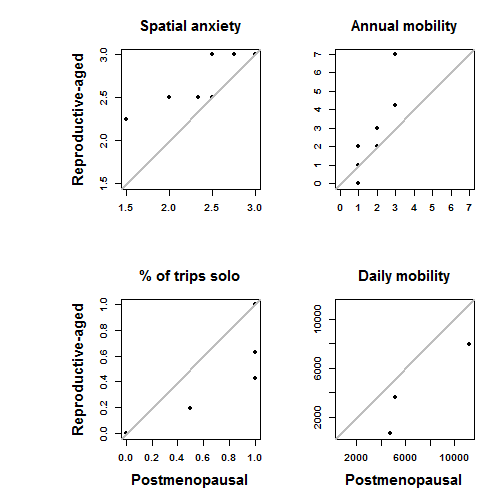
\includegraphics[width=0.75\textwidth]{QQ_pst}
\caption{Please write your figure caption here}
\label{fig:meno}       % Give a unique label
\end{figure}


	\subsection{Lactation and gestation effects}
	\label{sec:3.3}
	
Women with an unweaned child at the time of testing responded slightly more quickly and accurately to the mental rotation task than other women of reproductive age, but the differences are small enough to easily be explained by random chance (see Table \ref{tab:lact}).  The sample includes only three pregnant women, but two of them were among the eleven women to obtain a perfect score on the mental rotation task.  This difference in accuracy is not statistically significant, but their advantage over other women in response time is statistically significant despite the weak power of the study (see Table \ref{tab:preg}).  

Postpartum women also performed considerably better than other reproductive-aged women on the pointing accuracy measure of navigational skill.  However, the difference is not statistically significant, and a larger sample may be needed to assess the relationship between navigation ability and lactation.  The three pregnant women were less accurate than the set of reproductive-aged women who were neither pregnant nor lactating. 

Consistent with the fertility and parental care hypothesis, postpartum women self-reported higher spatial anxiety than other reproductive-aged women.  Only two of the pregnant women responded to the spatial anxiety questionnaire.  These women reported lower spatial anxiety than the average reproductive-aged women who were neither pregnant nor lactating.

\begin{table}[h!]
\caption{Postpartum}
\label{tab:lact}  
\begin{tabular}{llllllll}
\hline\noalign{\smallskip}
& \multicolumn{2}{c}{Lactating} && \multicolumn{2}{c}{Cycling} && \\
Measure & \emph{N} & \emph{M(SD)} && \emph{N} & \emph{M(SD)} && \emph{p} \\
\noalign{\smallskip}\hline\noalign{\smallskip}
Mental rotation (accuracy) & 21 & 83.7\%(17.5\%) && 14 & 81.0\%(14.6\%) && .627 \\
Mental rotation (time) & 21 & 5.38(1.68) && 14 & 5.80(1.27) && .404 \\
Pointing error & 24 & 16.73$^{\circ}$(8.02$^{\circ}$) && 17 & 20.97$^{\circ}$(12.37$^{\circ}$) && .227 \\
Spatial anxiety & 12 & 2.83(0.25) && 5 & 2.60(0.22) && .092 \\
Annual visits & 19 & 2.84(1.89) && 12 & 1.33(1.15) && .01 \\
Solo visit \% & 19 & 22.0\%(33.7\%) && 9 & 22.2\%(36.3\%) && .984 \\
Daily mobility (km) & 19 & 3.78(1.36) && 5 & 3.71(2.82) && .960 \\
\noalign{\smallskip}\hline
\end{tabular}\par
\bigskip
Means and standard deviations for lactating women and reproductive-aged women who are neither lactating nor pregnant in each of the listed measures. Final column gives the \emph{p-value} for a Chi-squared test comparing the two groups.  ``Cycling'' refers to reproductive-aged women in any stage other than lactation or gestation.  
\end{table}	

The fertility and parental care hypothesis predicts that women will curtail mobility due to the risks and caloric costs of travel.  Surprisingly, Twe women with unweaned children visited more than twice as many locations in the past year as women who were neither pregnant nor lactating.  Unlike the highly mobile postpartum mothers, the four pregnant women remained home most of the past year, and none of them made a single trip unaccompanied.\footnote{One complication with the annual mobility data is that women may have moved through more than one of the relevant reproductive stages in the past year. One woman who was breastfeeding at the time of her interview reported two visits away from home, both of which took place while she was pregnant.  None of the other lactating women reported a unique visit that occurred prepartum.  Similarly, none of the pregnant women reported unique visits that took place before they were pregnant, and none of the other women reported unique visits that took place before their youngest child was weaned.  For this measure, we moved the one problematic case from the ``lactating'' to the ``gestating'' group.}


% For one-column wide figures use
\begin{figure}[!htb]
  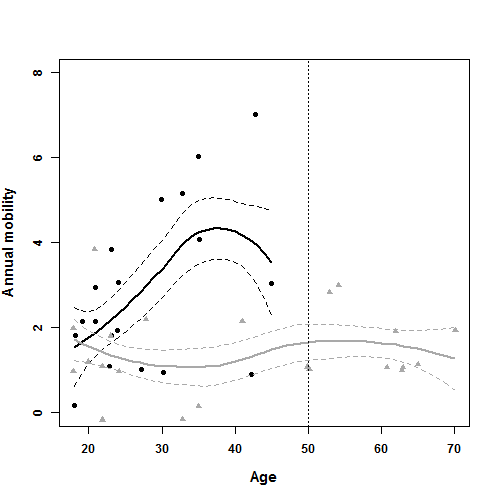
\includegraphics[width=0.75\textwidth]{lactmob}
\caption{The grey triangles and corresponding grey loess lines plot the number of unique annual visits reported by women who were neither pregnant nor lactating at all ages.  The black circles and corresponding loess lines plot the number of unique annual visits reported by women who were breastfeeding.  The dashed lines show one standard deviation on either side of the respective loess lines.  The dotted line notes 50 years, after which all women are expected to be postmenopausal.}
\label{fig:lactmob}       % Give a unique label
\end{figure}


\begin{table}[h!]
\caption{Gestation}
\label{tab:preg}  
\begin{tabular}{llllllll}
\hline\noalign{\smallskip}
& \multicolumn{2}{c}{Pregnant} && \multicolumn{2}{c}{Cycling} && \\
Measure & \emph{N} & \emph{M(SD)} && \emph{N} & \emph{M(SD)} && \emph{p} \\
\noalign{\smallskip}\hline\noalign{\smallskip}
Mental rotation (accuracy) & 3 & 92.6\%(12.8\%) && 14 & 81.0\%(14.6\%) && .255 \\
Mental rotation (time) & 3 & 3.7(0.51) && 14 & 5.80(1.27) && .001 \\
Pointing error & 3 & 24.98$^{\circ}$(8.09$^{\circ}$) && 17 & 20.97$^{\circ}$(12.37$^{\circ}$) && .611 \\
Spatial anxiety & 2 & 2.38(0.18) && 5 & 2.60(0.22) && .274 \\
Annual visits & 4 & 1.25(0.96) && 12 & 1.33(1.15) && .891 \\
Solo visit \% & 2 & 0\%(0\%) && 9 & 22.2\%(36.3\%) && .104 \\
Daily mobility (km) & 3 & 4.24(3.06) && 5 & 3.71(2.82) && .820 \\
\noalign{\smallskip}\hline
\end{tabular}\par
\bigskip
Means and standard deviations for pregnant women and reproductive-aged women who are neither lactating nor pregnant in each of the listed measures. Final column gives the \emph{p-value} for a Chi-squared test comparing the two groups.  ``Cycling'' refers to reproductive-aged women in any stage other than lactation or gestation. 
\end{table}	

	\subsection{Spatial ability, ranging, and the interaction with sex}
	\label{sec:3.4}
The fertility and parental care hypothesis predicts a positive relationship between spatial-cognitive ability and mobility. This expectation is shared with the other prominent theories linking spatial cognition to travel-based fitness effects, however, the others focus on this relationship in men rather than women.  Thus, looking at which sexes travel more in response to variance in spatial ability may help discriminate between possible explanations.	

\begin{table}[!tb]
\caption {Annual mobility and Spatial Cognition}
\label{tab:wm_spacemob}
  \centering
  \begin{tabular}{| l  ll  ll  ll  l |} 
    \hline   
  & \multicolumn{6}{c}{Independent Variables}& \\    
  & \multicolumn{2}{c}{MR} & \multicolumn{2}{c}{Male(1$|$0)} & \multicolumn{2}{c}{Male(1$|$0):MR} & $R^2$ \\
  & $Std. \beta$ & $Std. Err$ & $Std. \beta$ & $Std. Err$ & $Std. \beta$ & $Std. Err$  & \\
  Model 1 & 0.207\phantom{**} & 0.134\phantom{**} & & & & & 0.036\phantom{**} \\
  Model 2 & 0.262 & 0.137\phantom{**} & 0.331** & 0.114\phantom{**} & .300* & 0.131\phantom{**} & 0.222\\
  \hline 
  \end{tabular}  
{Coefficient for a linear model with mental rotation accuracy as a lone predictor of annual visits (``Model 1''), and a binary sex variable included as an interaction term with mental rotation accuracy (``Model 2'').  * \emph{p} $<$ .05; ** \emph{p} $<$  .01 }
\end{table}

Mental rotation performance as a lone predictor in a linear model is only weakly predictive of travel in the past year, and is not a statistically significant improvement over a null model ($M_{null} | M_1$, $\chi^2(1, 98) = 2.348, p = 0.121$).  However, including sex as an interaction effect dramatically improves model performance ($M_1 | M_2$, $\chi^2(2, 98) = 12.091, p = 0.0006$).  Interestingly, the effect runs in the opposite direction of expectations drawn from the fertility and parental care hypothesis.  Men, but not women, with higher spatial ability appear to travel more broadly (see Figure \ref{fig:mw_acctot} and Table \ref{tab:wm_spacemob}).  This is consistent with findings in a previous study using a different measure of mental rotation (cite me).

% For one-column wide figures use
\begin{figure}[!htb]
  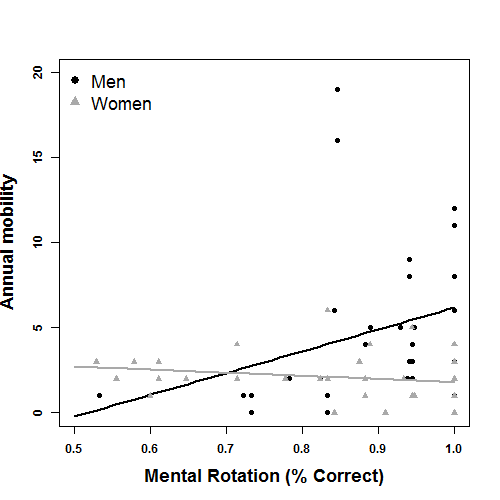
\includegraphics[width=0.75\textwidth]{mw_acctot}
\caption{Plot fitting the unstandardized coefficients for Model 2 described in \ref{tab:wm_spacemob}. Grey triangles and corresponding line demonstrate the relationship between performance on the mental rotation task and annual range.  Black triangles and corresponding line show the same relationship for men.}
\label{fig:1}       % Give a unique label
\end{figure}

\section{Discussion}
\label{sec:4}

The observed sex differences across spatial cognition, navigation, spatial anxiety, annual mobility and daily mobility are all consistent with the fertility and parental care hypothesis.  Men outperformed women in the spatial-cognitive and navigational tasks, reported lower spatial anxiety, and traveled further at both scales.  However, all of these predictions apply equally well to the other prominent theories linking these traits in an evolutionary framework.  

The only area of this study that consistently fits expectations uniquely drawn from the fertility and parental care hypothesis is the spatial anxiety measure.  Postmenopausal women reported lower spatial anxiety than reproductive-aged women, and among the latter group, women with an unweaned infant reported higher spatial anxiety.  Unfortunately, both of these tests lack statistical power.  We may expect increased anxiety during key periods of reproduction to be adaptive even if limiting travel is not the function.  In addition to concerns about travel, anxiety should promote hyper-vigilance to threats like children being bitten by scorpions, consuming harmful substances, or falling into fires (a common source of injury for Twe and Himba children).  This study specifically used a measure targeting the dangers of travel, but the results could simply be picking up on general anxiety.

The mobility data also shows intriguing trends in the difference between postmenopausal and reproductive-aged women, with the older women moving much more on a daily basis and making a higher percentage of their annual visits abroad without accompaniment.  These trends are consistent with the fertility and parental care hypothesis but again are observed in a very small sample.

Interestingly, one of the strongest findings of the study actually runs in the opposite direction of the fertility and parental care hypothesis.  Despite the postpartum period being the most vulnerable time in a woman's life, and higher self-reported spatial anxiety among nursing Twe mothers, these women traveled to more than twice as many unique locations as other reproductive-aged (and not pregnant) women in the past year. 

We asked about the purpose of each trip reported in the annual mobility interviews.  This information allows us to examine some potential explanations for the surprisingly high rate of postpartum travel.  The data may be capturing women returning to their natal community to seek the childcare assistance of their mothers.  This explanation follows from recent work showing exactly that pattern among a nearby Himba community  \citep{scelza2011female}.  However, none of the cases in our data are consistent with this explanation.  This may not be surprising, since the majority of Twe women already live with their mothers and other close kin \citep{vashro2014residence}.  

Instead of traveling to visit parents and siblings, the stated reason for many of the postpartum women's travel was to visit extended kin.  For example, two sisters, each with an unweaned child, traveled together approximately 160 kilometers through an unfamiliar region to visit a maternal aunt they had not seen since childhood.  Overall, 38.2\% (21 out of 55 trips) of the visits reported by women with unweaned children were targeted social visits to extra-nuclear kin, while only 5\% (2 out of 40) of the visits reported by reproductive-aged women at other reproductive stages were of that nature.  Extended kin networks are the primary safety net among the Twe.  Women with infants may be more successful in soliciting immediate assistance from relatives, and in several cases the explicit purpose of the trip was to beg for food or small-stock.  In addition, mothers may want to introduce their new infants to relatives to begin forming a strong kinship bond that will prove useful in the future.  If these incentives are strong enough, they could outweigh the risks of travel (though they may not have in a more dangerous past).  In addition, traveling long distances on foot to visit family may not be an energetic cost if you are ultimately eating from a relative's pot as a guest, rather than spending the day laboring to produce your next meal.

Another finding that poses a challenge to the fertility and parental care hypothesis was that there is a positive relationship between spatial ability and travel in the past year among men but not women.  This is consistent with previous work in the same population \citep{vashro2014spatial}.  Furthermore, a study among urban Canadians found a positive correlation between home-range size and mental rotation among men and not women \citep{ecuyer2004spatial}.  The consistency of this finding makes it difficult to highlight the importance of this relationship for women.

%Interested in future work looking at the volume and function of women's postpartum mobility in other populations, including the US.

%Looking across the entire life-cycle, it is true that women's estrogen level rise as they enter reproductive maturity (is this tru?), and fall after menopause.  This lines up with the theory linking decreased mobility as a risk reduction strategy that is mediated by estrogen.  However, looking within women of reproductive age the pattern of estrogen cycles is more difficult to link with at least a simple version of risk reduction.  The problem is that women's estrogen level drop post-partum.  The team between  birth and weaning is likely \emph{the} time when the concerns highlighted by the fertility and parental care hypothesis should be most important. Instead, at least among mice, this period is associated with improved performance in maze tasks ans increased range (nest visits?... check this). 


%\begin{acknowledgements}
%If you'd like to thank anyone, place your comments here
%and remove the percent signs.
%\end{acknowledgements}

% BibTeX users please use one of
%\bibliographystyle{spbasic}      % basic style, author-year citations
%\bibliographystyle{spmpsci}      % mathematics and physical sciences
%\bibliographystyle{spphys}       % APS-like style for physics
%\bibliography{}   % name your BibTeX data base

% Non-BibTeX users please use
\bibliography{bfeed_refs}
\bibliographystyle{spbasic}      % basic style, author-year citations

\end{document}
% end of file template.tex
